\section{Method}
\label{sec:method}

We formulate \modelname{} as a coarse-to-fine model for 3D hand-motion forecasting. The method combines a deterministic frequency-domain predictor with a conditional diffusion model over residual future motion. Its central design choice is to represent uncertainty in a spatio-spectral residual space shaped jointly by articulated hand structure and frequency-dependent future motion modes. An overview of the full architecture is shown in Fig.~\ref{fig:model_overview}.

\begin{figure*}[t]
    \centering
    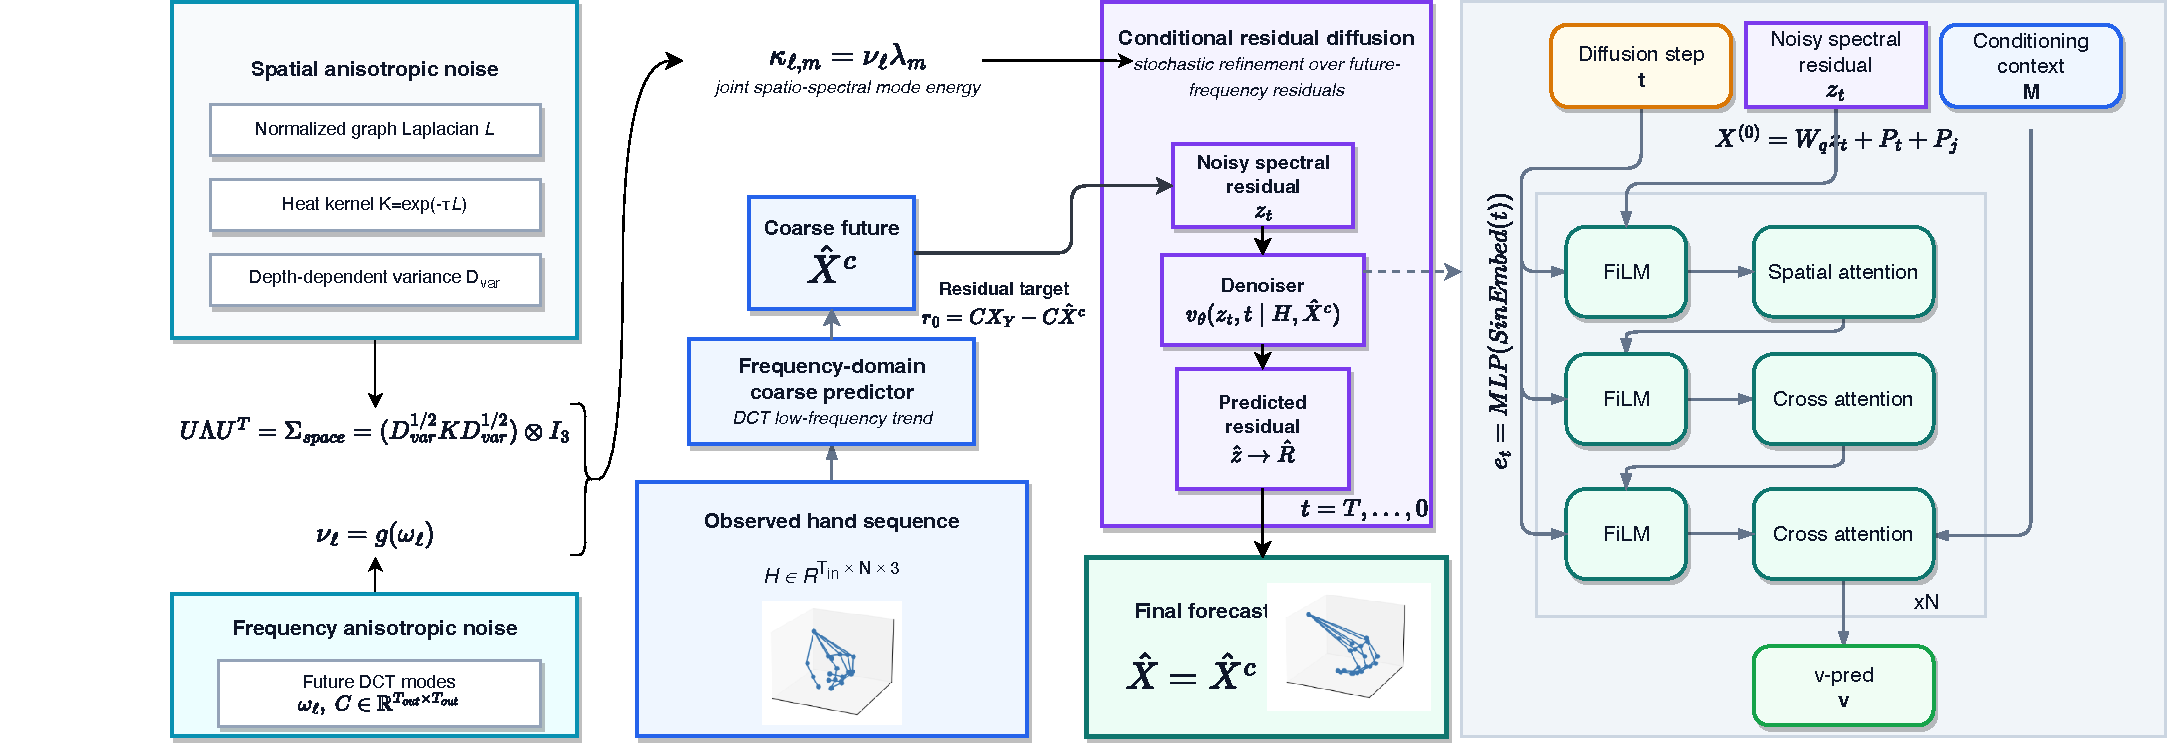
\includegraphics[width=\textwidth]{figures/model_freq.pdf}
    \caption{Overview of \modelname{}. The model first predicts a coarse future in the frequency domain, then refines it with conditional residual diffusion in a spatio-spectral space structured by articulated hand topology and future-frequency anisotropy.}
    \label{fig:model_overview}
\end{figure*}

\subsection{Problem Formulation}
\label{sec:method_problem}

Let
\[
H \in \mathbb{R}^{T_{\mathrm{in}} \times N \times 3},
\qquad
Y \in \mathbb{R}^{T_{\mathrm{out}} \times N \times 3}
\]
denote the observed and future 3D hand trajectories, where $T_{\mathrm{in}}$ and $T_{\mathrm{out}}$ are the observation and prediction horizons and $N$ is the number of joints. We use the flattened representations
\[
X_H \in \mathbb{R}^{T_{\mathrm{in}} \times F},
\qquad
X_Y \in \mathbb{R}^{T_{\mathrm{out}} \times F},
\qquad
F = 3N.
\]

The forecasting problem is decomposed into two stages. First, a deterministic branch predicts a coarse future $\hat{X}^{c}$. Second, a stochastic refinement branch models the residual motion that remains after this coarse prediction has been formed.

\subsection{Coarse Frequency-Domain Forecasting}
\label{sec:method_coarse}

The coarse branch operates in a DCT representation of the full observation--prediction window. Let
\[
T = T_{\mathrm{in}} + T_{\mathrm{out}}
\]
and let $\tilde{X} \in \mathbb{R}^{T \times F}$ denote the temporally extended sequence obtained by appending a simple continuation of the observed motion to the input history. We project this sequence onto a low-frequency DCT basis,
\[
Z_{\mathrm{low}} = C_{\mathrm{low}} \tilde{X},
\]
where $C_{\mathrm{low}}$ contains the low-frequency rows of the orthonormal DCT matrix over the full window.

A sequence predictor then operates on this compact frequency representation and estimates the dominant spectral structure of the full trajectory. Drawing inspiration from SiMLPe \cite{Guo2023SiMLPe}, which provides a strong and simple frequency-domain forecasting baseline, we instantiate this predictor as a stack of temporal MLP layers over the DCT coefficients. The predicted low-frequency coefficients are mapped back to the time domain and restricted to the prediction horizon, producing the coarse future
\[
\hat{X}^{c} \in \mathbb{R}^{T_{\mathrm{out}} \times F}.
\]
This stage captures the large-scale and relatively stable components of the future motion while leaving the remaining uncertainty to the residual model.

Since the stochastic branch acts on future-frequency residuals, we also define the DCT representation of the coarse future over the prediction horizon:
\[
\hat{Y}^{c}_{f} = C \hat{X}^{c},
\]
where $C \in \mathbb{R}^{T_{\mathrm{out}} \times T_{\mathrm{out}}}$ is the orthonormal DCT matrix over the prediction horizon.

\subsection{Spatial and Frequency Anisotropy}
\label{sec:method_anisotropy}

\paragraph{Spatial prior.}
The spatial prior is defined from the articulated hand topology. We consider a hand graph
\[
G = (V,E),
\]
where the nodes represent joints and the edges encode kinematic adjacency. To represent non-uniform residual variability across the hand, we assign depth-dependent variance weights to the joints. Let
\[
D_{\mathrm{var}} = \operatorname{diag}(d_1,\dots,d_N)
\]
be the diagonal matrix of jointwise variance weights. These weights act as a nodewise amplitude prior: more constrained joints receive smaller variance weights, whereas more mobile articulators receive larger ones.

To couple neighboring joints, we define a graph-smooth covariance factor from the hand topology. Let \(A\) be the adjacency matrix of the hand graph and \(D_g\) its degree matrix. We form the normalized graph Laplacian \cite{chung1997spectral}
\[
L = I - D_g^{-1/2} A D_g^{-1/2},
\]
and the associated heat kernel
\[
K = \exp(-\delta L),
\]
where \(\delta>0\) controls the smoothing scale on the hand graph. This kernel is symmetric positive definite and diffuses covariance over the graph, so that nearby kinematic neighbors receive stronger cross-joint coupling than distant joints.

We combine graph smoothness and heteroskedastic joint variance at the node level as
\[
\Sigma_{\mathrm{node}}
=
D_{\mathrm{var}}^{1/2} K D_{\mathrm{var}}^{1/2},
\]
then lift this covariance to 3D coordinates through
\[
\Sigma_{\mathrm{space}} = \Sigma_{\mathrm{node}} \otimes I_3.
\]
The heat-kernel factor determines how covariance spreads over the hand graph, while \(D_{\mathrm{var}}\) controls the marginal uncertainty scale at each joint. This construction yields spatial residual modes that are simultaneously graph-smooth and non-uniform across articulators.

We write the eigendecomposition of the resulting spatial covariance as
\[
\Sigma_{\mathrm{space}} = U \Lambda U^\top,
\]
where $U$ is the spatial spectral basis and
\[
\Lambda = \operatorname{diag}(\lambda_1,\dots,\lambda_{F})
\]
contains the spatial mode energies. This basis defines the articulated residual directions used by the diffusion model.

\paragraph{Frequency anisotropy.}
The stochastic branch also distinguishes between future motion modes of different frequency. Let
\[
\omega_\ell, \qquad \ell=1,\dots,T_{\mathrm{out}},
\]
index the future DCT modes. We assign a nonnegative frequency weight to each mode,
\[
\nu_\ell = g(\omega_\ell),
\]
where $g(\cdot)$ is a monotone spectral weighting function. In the present model, this weighting plays the role of a temporal or frequency anisotropy term: lower- and higher-frequency future modes need not be corrupted at the same rate.

The spatial and frequency components are combined into a spatio-spectral anisotropic schedule. For frequency mode $\ell$ and spatial mode $m$, we define the joint mode energy
\[
\kappa_{\ell,m} = \nu_\ell \lambda_m.
\]
These joint energies determine how strongly each residual mode is noised during diffusion. As a result, uncertainty is not represented isotropically: it is structured both across articulated hand directions and across future frequency modes.
Intuitively, this formulation changes the corruption schedule by no longer treating all residual coefficients equally. Residual modes that vary more rapidly over the forecast horizon receive larger frequency weights and are therefore noised more aggressively. On the spatial side, modes with larger prior residual variability---typically those emphasizing more mobile articulated regions while remaining compatible with the hand graph---also receive faster corruption. Conversely, smoother and more topology-consistent residual modes retain signal longer during the forward process.

\subsection{Conditional Residual Diffusion}
\label{sec:method_diffusion}

The stochastic branch models residual motion in the future frequency domain. Let
\[
r_0 = C X_Y - C \hat{X}^{c}
\]
denote the clean future-frequency residual over the full hand-coordinate representation. Rather than diffusing this residual directly in the original coefficient coordinates, we express it in the spatial spectral basis induced by the covariance prior:
\[
z_0 = r_0 U.
\]
Here the DCT matrix $C$ acts along the temporal prediction axis, while the spatial basis $U$ acts along the $F$-dimensional hand-coordinate axis. Therefore $z_0 \in \mathbb{R}^{T_{\mathrm{out}} \times F}$ remains indexed jointly by future frequency and spatial residual mode.

Given a diffusion timestep $t$, the noised residual state is defined by mode-dependent perturbation in this spectral space:
\[
z_t =
\sqrt{\bar{\alpha}_t}\odot z_0
+
\sqrt{1-\bar{\alpha}_t}\odot \epsilon,
\qquad
\epsilon \sim \mathcal{N}(0,I),
\]
where the cumulative attenuation factors are applied elementwise over the spatio-spectral modes and depend on the anisotropic schedule introduced above. Hence, residual directions associated with different articulated structures or different future frequency modes are corrupted at different rates.

The denoiser is conditioned on the observed history and on the coarse future. Its role is to predict the standard $v$ target associated with the pair $(z_0,\epsilon)$ at timestep $t$, rather than reconstructing the clean residual directly. This choice yields a conditional residual diffusion model whose stochastic component is centered around the coarse forecast instead of replacing it.

After denoising, the residual is mapped back from the spatial spectral basis as $\hat{r}=\hat{z}U^\top$, inverted from the future DCT representation, and added to the coarse trajectory. The final forecast is thus
\[
\hat{X} = \hat{X}^{c} + \hat{R},
\]
where $\hat{R}$ is the decoded residual trajectory, expressed in the same trajectory coordinate system as the coarse branch.

\begin{proposition}[Validity of the spatio-spectral forward process]
\label{prop:ss_validity}
For the spatio-spectral forward process introduced above, the following properties hold:
\begin{enumerate}
    \item the forward noising process is admissible, with nonnegative variance in every spatio-spectral mode;
    \item the induced process in the residual coordinates is linear-Gaussian;
    \item the process is Markov, with mode-wise one-step transitions; and
    \item the process is compatible with standard $v$-prediction.
\end{enumerate}
\end{proposition}

This proposition formalizes the fact that the proposed diffusion process is a valid anisotropic forward model over future-frequency residuals. A proof is provided in the supplementary appendix.

\subsection{Training and Inference}
\label{sec:method_training}

\modelname{} is trained in two phases. The first phase optimizes the coarse forecasting branch so that it captures the dominant predictive structure of future hand motion. The second phase trains the residual diffusion branch while allowing the coarse predictor to remain jointly refinable after the initial warmup. This preserves consistency between the deterministic stage and the stochastic refinement stage, rather than treating the coarse forecast as a fixed external module.

At inference time, the model first predicts the coarse future trajectory, then forms its future-frequency representation, samples a residual correction through iterative denoising in spatio-spectral space, and finally reconstructs the future hand trajectory by adding the decoded residual to the coarse prediction. Optimization details, schedule parameters, and architecture hyperparameters are deferred to the experimental section.
